\documentclass[12pt]{tcc} 

\usepackage[brazil]{babel} 
\usepackage[T1]{fontenc}
\usepackage[hidelinks]{hyperref}
\usepackage[pt-BR]{datetime2}
\usepackage{url}
\usepackage[portuguese,ruled,linesnumbered,algochapter,titlenumbered]{algorithm2e}
\usepackage[normalem]{ulem}
\usepackage{listings}
\usepackage{tikz}
\usepackage[justification=centering]{caption}
\usepackage{placeins}
\usepackage{tabularx} 
\usetikzlibrary{shapes, arrows, positioning, fit}
%code style
\usepackage{float}
\usepackage{blindtext}
\usepackage[dvipsnames]{xcolor}
\usepackage{minted}
\usemintedstyle{borland}
\definecolor{command-line}{rgb}{0.85,0.85,0.9}
\definecolor{php-code}{rgb}{1,1,1}

% Color definition %
\definecolor{bash_main_commands}{rgb}{0.0, 0.0, 1.0}

\usepackage{lipsum}
\lstset{
  language        = php,
  basicstyle      = \small\ttfamily,
  keywordstyle    = \color{blue},
  keywords    ={__halt_compiler, abstract, and, array,
                    as, break,  callable,   case,   catch, class,
                    clone,  const,  continue,   declare,    default,
                    die,    do, echo,   else,   elseif,
                    empty,  enddeclare, endfor, endforeach, endif,
                    endswitch,  endwhile,   eval,   exit,   extends,
                    final,  finally,    for,    foreach,    function,
                    global, goto, if,   implements, include,
                    include_once,   instanceof, insteadof,
                    interface,  isset, list,    namespace,
                    new,    or, print, private, protected,  public,
                    require,    require_once, return,   static,
                    switch, throw,  trait, try, unset, use, var,
                    while,  xor,    yield, string, int, object, closure
  },
  stringstyle     = \color{red},
  identifierstyle = \color{OliveGreen},
  commentstyle    = \color{gray},
  emph            =[1]{php},
  emphstyle       =[1]\color{violet},
  emph            =[2]{if,and,or,else, bool, null},
  emphstyle       =[2]\color{blue},
  emph            =[3]{Core, Abstractions, Model, App, Models, User, Database, Query, SelectBuilder, JoinBuilder, HavingBuilder, Hash, Post, Team, Schema, TableBuilder, ChangeTableBuilder, Factories, UserFactory, Factory, DateTime, UserSeeder, Seeder, UserController, Uri, CreatePostsTable, Migration,  Enterprise, Phone, Test   },
  emphstyle       =[3]\color{orange},
  emph            =[4]{User, git, clone},
  emphstyle       =[4]\color{orange},
  emph            =[5]{index, find, get, where, orWhere, whereNot, whereBetween, whereNotBetween, whereIsNull, whereIsNotNull, whereAll, from, column, whereNotIn, whereExists, whereIn, when, on, orderBy, groupBy, limit, having, or, and, first, last, insert, hashPassword, update, delete, abstract, create, and, array,
                    as, break,  callable,   case,   catch, class,
                    clone,  const,  continue,   declare,    default,
                    die,    do, echo,   else,   elseif,
                    empty,  enddeclare, endfor, endforeach, endif,
                    endswitch,  endwhile,   eval,   exit,   extends,
                    final,  finally,    for,    foreach,    function,
                    global, goto, if,   implements, include,
                    include_once,   instanceof, insteadof,
                    interface,  isset, list,    namespace,
                    new,    or, print, private, protected,  public,
                    require,    require_once, return,   static,
                    switch, throw,  trait, try, unset, use, var,
                    while,  xor,    yield, string, int, object, closure, hasOne, hasMany, hasManyThrough, belongsTo, 
                     hasOneThrough,
                    belongsToMany, trace, enableTraceMode,
                    dateTime, varchar, id, primaryKey, autoIncrement, foreignKey, unique, visible, fullText, alter, dropColumn, dropConstraint, dropIndex, notNull, change, drop, faker, name, safeEmail. currentDateTime, self, void, factory, view, getRootPath, bigInt, timestamp},
  emphstyle       =[5]\color{blue},
  numbers=left,
  stepnumber=1,  
  numberfirstline=true,
  numberstyle=\footnotesize,
  upquote=true,
  showlines=true,
  showspaces=false,
  captionpos=b
  }

  \lstset{
  language        = bash,
  basicstyle      = \small\ttfamily,
  keywordstyle    = \color{blue},
  keywords    ={__halt_compiler},
  stringstyle     = \color{red},
  identifierstyle = \color{black},
  commentstyle    = \color{gray},
  emph            =[1]{git, composer, php, cosmo, APP_NAME, APP_ENV, APP_URL, APP_LOCALHOST_SERVER_PORT, DB_CONNECTION, DB_HOST, DB_PORT, DB_DATABASE, DB_USERNAME, DB_PASSWORD, DB_CHARSET},
  emphstyle       =[1]\color{bash_main_commands},
  emph            =[2]{help, api, step, filename},
  emphstyle       =[2]\color{orange},
  numbers=left,
  stepnumber=1,  
  numberfirstline=true,
  numberstyle=\footnotesize,
  upquote=true,
  showlines=true,
  showspaces=false,
  captionpos=b
  }

\colorlet{punct}{red!60!black}
\definecolor{background}{HTML}{FFFFFF}
\definecolor{delim}{RGB}{20,105,176}
\colorlet{numb}{magenta!60!black}

\usepackage{xcolor}

\newboolean{showcomments}
\setboolean{showcomments}{true}
\ifthenelse{\boolean{showcomments}}
 { \newcommand{\mynote}[3]{
      \fbox{\bfseries\sffamily\scriptsize#1}
        {\small$\blacktriangleright$\textsf{\textcolor{#3}{{\em #2}\bf }}$\blacktriangleleft$}}}
        { \newcommand{\mynote}[2]{}}
\newcommand{\pantoja}[1]{\mynote{Pantoja}{#1}{blue}}
\newcommand{\attention}[1]{\mynote{Atenção}{#1}{red}}
\newcommand{\modify}[1]{\mynote{Ajustes}{#1}{orange}}
\newcommand{\john}[1]{\mynote{Jonh}{#1}{brown}}

\lstdefinestyle{mystyle}{
    basicstyle=\normalfont\ttfamily,
    numbers=left,
    numberstyle=\scriptsize,
    stepnumber=1,
    numbersep=1pt,
    showstringspaces=false,
    breaklines=true,
    postbreak=\mbox{\textcolor{red}{$\hookrightarrow$}\space},
    frame=lines,
    backgroundcolor=\color{background}
}
\lstset{style=mystyle}

\lstdefinelanguage{json}{0
    literate=
     *{0}{{{\color{numb}0}}}{1}
      {1}{{{\color{numb}1}}}{1}
      {2}{{{\color{numb}2}}}{1}
      {3}{{{\color{numb}3}}}{1}
      {4}{{{\color{numb}4}}}{1}
      {5}{{{\color{numb}5}}}{1}
      {6}{{{\color{numb}6}}}{1}
      {7}{{{\color{numb}7}}}{1}
      {8}{{{\color{numb}8}}}{1}
      {9}{{{\color{numb}9}}}{1}
      {:}{{{\color{punct}{:}}}}{1}
      {,}{{{\color{punct}{,}}}}{1}
      {\{}{{{\color{delim}{\{}}}}{1}
      {\}}{{{\color{delim}{\}}}}}{1}
      {[}{{{\color{
delim}{[}}}}{1}
      {]}{{{\color{delim}{]}}}}{1},
}

\lstdefinelanguage{Jason}{
    literate=
     *{0}{{{\color{numb}0}}}{1}
      {1}{{{\color{numb}1}}}{1}
      {2}{{{\color{numb}2}}}{1}
      {3}{{{\color{numb}3}}}{1}
      {4}{{{\color{numb}4}}}{1}
      {5}{{{\color{numb}5}}}{1}
      {6}{{{\color{numb}6}}}{1}
      {7}{{{\color{numb}7}}}{1}
      {8}{{{\color{numb}8}}}{1}
      {9}{{{\color{numb}9}}}{1}
      {:}{{{\color{punct}{:}}}}{1}
      {;}{{{\color{punct}{;}}}}{1}
      {,}{{{\color{punct}{,}}}}{1}
      {\{}{{{\color{delim}{\{}}}}{1}
      {\}}{{{\color{delim}{\}}}}}{1}
      {[}{{{\color{delim}{[}}}}{1}
      {]}{{{\color{delim}{]}}}}{1}
      {<-}{{{\color{punct}{<-}}}}{2}
      {.}{{{\color{punct}{.}}}}{1},
}

\lstdefinelanguage{Java}{
    literate=
     *{0}{{{\color{numb}0}}}{1}
      {1}{{{\color{numb}1}}}{1}
      {2}{{{\color{numb}2}}}{1}
      {3}{{{\color{numb}3}}}{1}
      {4}{{{\color{numb}4}}}{1}
      {5}{{{\color{numb}5}}}{1}
      {6}{{{\color{numb}6}}}{1}
      {7}{{{\color{numb}7}}}{1}
      {8}{{{\color{numb}8}}}{1}
      {9}{{{\color{numb}9}}}{1}
      {:}{{{\color{punct}{:}}}}{1}
      {;}{{{\color{punct}{;}}}}{1}
      {,}{{{\color{punct}{,}}}}{1}
      {\{}{{{\color{delim}{\{}}}}{1}
      {\}}{{{\color{delim}{\}}}}}{1}
      {[}{{{\color{delim}{[}}}}{1}
      {]}{{{\color{delim}{]}}}}{1}
      {<-}{{{\color{punct}{<-}}}}{2}
      {.}{{{\color{punct}{.}}}}{1},
}

% Desenho de X
\newcommand{\tikzcmark}{
\tikz[scale=0.23] {
    \draw[line width=0.7,line cap=round] (0.25,0) to [bend left=10] (1,1);
    \draw[line width=0.8,line cap=round] (0,0.35) to [bend right=1] (0.23,0);
}}

% Definições.
\usepackage{amsthm}
\newtheorem{definition}{Definição}

% Algoritmo
\newcommand{\spaceH}[1]{\ \ \ \ \ }
\newcommand{\spaceAction}[1]{\- \spaceH \spaceH \spaceH }

% As Figuras ficam armazenadas na pasta Figuras
\graphicspath{{./figures/}}

% Informações do trabalho
\newcommand\dtitle{A Importância das Ferramentas Open Source no Desenvolvimento de Pipelines de Dados}
\newcommand\dauthor{Pedro Medeiros Pereira Carvalho}
\newcommand\dadvisor{Diego Cardoso Borda Castro}

% Definição de acronimos

\DeclareAcronym{api}{
    short = API,
    long  = Application Programming Interface
}

\DeclareAcronym{bi}{
    short = BI,
    long  = Business Intelligence
}

\DeclareAcronym{cli}{
    short = CLI,
    long  = Command-Line Interface
}

\DeclareAcronym{csrf}{
    short = CSRF,
    long  = Cross-site Request Forgery
}

\DeclareAcronym{dl}{
    short = DL,
    long  = Data Lake
}

\DeclareAcronym{dsr}{
    short = DSR,
    long  = Design Science Research
}

\DeclareAcronym{dw}{
    short = DW,
    long  = Data Warehouse
}

\DeclareAcronym{etl}{
    short = ETL,
    long  = {Extract, Transform, Load}
}

\DeclareAcronym{html}{
    short = HTML,
    long  = HyperText Markup Language
}

\DeclareAcronym{http}{
    short = HTTP,
    long  = Hypertext Transfer Protocol
}

\DeclareAcronym{iot}{
    short = IoT,
    long  = Internet of Things
}

\DeclareAcronym{llm}{
    short = LLM,
    long  = Large Language Model
}

\DeclareAcronym{npm}{
    short = NPM,
    long  = Node Package Manager
}

\DeclareAcronym{orm}{
    short = ORM,
    long  = Object-Relational Mapping
}

\DeclareAcronym{php}{
    short = PHP,
    long  = Hypertext Preprocessor
}

\DeclareAcronym{rr}{
    short = RR,
    long  = Rapid Review
}

\DeclareAcronym{sql}{
    short = SQL,
    long  = Structured Query Language
}

\DeclareAcronym{url}{
    short = URL,
    long  = Uniform Resource Locator
}

\DeclareAcronym{PMEs}{
    short = PMEs,
    long  = Pequenas e Médias Empresas
}

\DeclareAcronym{DSR}{
    short = DSR,
    long  = Design Science Research
}
\begin{document}
\pagenumbering{gobble}
\pagenumbering{roman}

\dcover

\dcoverback

\newpage
\dacknowledgment{
Upcoming...
}



\dresumo{
A criação de pipelines de dados por meio de soluções proprietárias apresenta algumas desvantagens competitivas, como a falta de transparência, a dependência de fornecedores e, principalmente, os altos custos. O \textit{software} de código aberto surge nesse contexto com um modelo de desenvolvimento descentralizado e colaborativo, que distribui o código-fonte publicamente, permitindo que qualquer pessoa possa usar, alterar e redistribuir como preferir, sem custo adicional. No entanto, o mercado ainda enfrenta desafios e resistências na adoção dessas soluções. Para enfrentar esse problema, este trabalho mapeou os principais \textit{softwares} livres utilizados no mercado para atividades de engenharia de dados, com o propósito de criar um catálogo de aplicações para construção de \textit{pipeline} de dados \textit{open source}. Com o intuito de demonstrar a viabilidade prática, foi desenvolvido um exemplo prático de \textit{pipeline} com algumas das ferramentas encontradas, desde a concepção inicial até a implementação final, aplicado a um cenário de coleta de informações sobre passagens aéreas para o Brasil, extraindo as informações de diferentes sites internacionais. A análise focou no impacto dessas ferramentas em termos de escalabilidade e desempenho, com o intuito de oferecer uma base técnica relevante para trabalhos acadêmicos e pequenas e médias empresas que buscam soluções eficientes e acessíveis, sem comprometer seus recursos.
}
{\textit{Pipeline} de Dados; \textit{Software} Livre; Engenharia de Dados}

\dabstract{
    The development of data pipelines utilising proprietary solutions entails several competitive drawbacks, including opacity, vendor dependency, and, crucially, elevated expenses. Open-source software arises inside this framework, characterised by a decentralised and collaborative development process that publicly disseminates the source code, permitting anybody to utilise, alter, and redistribute it at no additional cost. Nonetheless, the market continues to encounter obstacles and opposition in embracing these solutions. This study catalogued the primary free software utilised in the market for data engineering tasks, aiming to establish a repository of apps for constructing open-source data pipelines. To illustrate practical viability, a pipeline was constructed utilising various tools, from initial conception to final implementation, focused on gathering data regarding airline tickets to Brazil by extracting information from multiple international websites. The investigation examined the influence of these tools regarding scalability and performance, intending to furnish a pertinent technical foundation for academic research and small to medium-sized firms in pursuit of efficient and cost-effective solutions without depleting their resources.
}
{\textit{Data Pipeline}; \textit{Open Source}; \textit{Data Engineering}}
%\dtables

\tableofcontents
\newpage
\listoffigures


\pagenumbering{arabic}
\justifying
	
\chapter{Introdução}
\label{sec:introducao}

 Este capítulo tem como propósito introduzir o cenário em que se insere este trabalho de conclusão de curso, destacando sua motivação, os problemas investigados e os principais objetivos.

\section{Contextualização}

A era digital tem sido marcada por uma crescente geração de dados provenientes de diversas fontes, como redes sociais, dispositivos móveis, sensores de \textit{Internet of Things} (IOT) e sistemas transacionais. Nesse cenário, o conceito de \textit{Big Data} emerge como um paradigma essencial para lidar com essa grande quantidade de informações de maneira eficaz, possibilitando análises complexas e decisões baseadas em dados. Com o aumento da necessidade de extração de valor a partir desses dados, surgem arquiteturas e processos especializados como os \textit{pipelines} de dados, que são fluxos estruturados que extraem, transformam e carregam dados para ambientes de análise e decisão.

Historicamente, o ecossistema de dados nas organizações foi dominado pelas ferramentas proprietárias, ou seja, as fornecidas por grandes empresas, como Amazon, Microsoft e Google \cite{septian2019, reverseetl2022}. Estas soluções, juntamente com outras proprietárias, são explicitamente destacadas em comparação com alternativas de código aberto \cite{septian2019, reverseetl2022}. Essas soluções apresentam algumas limitações importantes, dentre elas os altos custos de licenciamento, dependência de fornecedores e restrições de customização. A precificação de muitas plataformas de dados em nuvem, especialmente as proprietárias, adota um modelo baseado no consumo, como o \textit{pay-per-use} ou custos por hora e nó de processamento \cite{murarka2024}. Este modelo de cobrança por uso e por escalabilidade automática para acomodar \textit{bursty workloads} \cite{murarka2024}, embora ofereça flexibilidade, introduz o custo de implementação e manutenção como um risco significativo no Big Data \cite{septian2019}. Além disso, a adoção dessas ferramentas pode se tornar um obstáculo para inovação e agilidade operacional, especialmente em contextos onde há necessidade de adaptação rápida a novas demandas de negócio ou escalabilidade. Em resposta à complexidade e ao risco de custos elevados inerentes aos modelos de precificação de plataformas proprietárias \cite{septian2019}, muitas organizações estão reorientando suas estratégias. Há uma busca crescente por alternativas que sejam mais acessíveis, modulares e flexíveis, sendo as soluções \textit{\textbf{open source}} destacadas como essenciais para permitir que até Pequenas e Médias Empresas (PMEs) enfrentem seus desafios de \textit{Big Data} \cite{septian2019, murarka2024}.

Para viabilizar as operações de dados de forma escalável e segura, e de maneira economicamente sustentável, especialmente em um cenário de constante crescimento do volume de dados, as ferramentas de código aberto \textit{open source} passaram a desempenhar um papel estratégico \cite{murarka2024, septian2019}. Plataformas como Hadoop, com seus componentes HDFS e MapReduce, tornaram-se essenciais no gerenciamento de conjuntos de dados em larga escala, provendo armazenamento distribuído e capacidades de processamento paralelo cruciais para a escalabilidade \cite{murarka2024}.

Essas ferramentas oferecem alternativas robustas e acessíveis às soluções proprietárias, permitindo que organizações de diferentes portes construam e personalizem suas próprias arquiteturas de dados. Além disso, a natureza colaborativa do \textit{software} \textit{open source} impulsiona a inovação contínua e facilita a integração com diferentes tecnologias, tornando-se um pilar fundamental na construção de \textit{pipelines} de dados modernos \cite{murarka2024, septian2019}. O uso de ferramentas como Apache Spark, por exemplo, oferece flexibilidade para acomodar tanto o processamento em lote quanto a manipulação de dados em tempo real, integrando-se de maneira robusta ao ecossistema de \textit{Big Data} \cite{murarka2024}.
    
Embora o uso de \textit{pipelines} de dados seja essencial para lidar com os desafios do \textit{Big Data} \cite{murarka2024}, muitas organizações enfrentam entraves significativos em sua implementação prática. Entre os principais desafios estão a complexidade da ingestão de dados em tempo real, a integração de fontes heterogêneas e a dificuldade em manter processos de transformação consistentes e escaláveis \cite{murarka2024, nwokeji2021}. Em particular, o ETL (Extract, Transform, Load) tradicional pode ser um processo de custo intensivo e é fundamentalmente uma abordagem unidirecional, não sendo capaz de movimentar dados para fora do \textit{data warehouse} \cite{nwokeji2021, reverseetl2022}.

Além disso, há uma ausência de diretrizes padronizadas que auxiliem na seleção, combinação e orquestração de ferramentas \textit{open source} de forma segura e eficiente. A falta de uma abordagem padronizada para modelar os processos e fluxos de trabalho do ETL é reconhecida como um desafio prevalente \cite{nwokeji2021}. Essa carência resulta na desorientação na escolha e na dificuldade de selecionar um ETL que esteja alinhado às necessidades específicas, preferências e interesses de cada organização \cite{boulahia2024}. Isso gera incertezas, retrabalho e adoções tecnológicas mal planejadas, resultando em arquiteturas pouco escaláveis ou difíceis de manter.

Diante desse cenário e dos problemas descritos, surge a questão de pesquisa deste trabalho: como ferramentas \textit{open source} podem ser utilizadas na construção de \textit{pipelines} de dados eficientes, escaláveis e acessíveis, e quais são seus impactos em comparação com soluções proprietárias. Visando auxiliar na resposta desta pergunta, este trabalho tem como principal objetivo analisar as ferramentas disponíveis para geração de um \textit{pipeline} de dados funcional e robusto, utilizando exclusivamente tecnologias livres, que seja equivalente aos \textit{pipelines} que são criados utilizando soluções proprietárias. Estudo que vai desde a coleta de dados brutos, realizando \textit{web scraping} de passagens aéreas de sites internacionais com destino ao Brasil, até a disponibilização para análise.

\section{Objetivos do Trabalho}
\label{sec:objetivo}

Este trabalho busca demonstrar a viabilidade técnica e econômica de \textit{pipelines} de dados baseados em ferramentas \textit{open source}, oferecendo uma alternativa às soluções proprietárias tradicionais. O foco recai sobre cenários onde orçamentos limitados e a necessidade de flexibilidade são críticos, tais como pequenas e médias empresas ou projetos acadêmicos. Para isso, é destacado:

\section{Justificativas da Abordagem \textit{Open Source} no \textit{Pipeline} de Dados}

A escolha pela construção de um \textit{pipeline} de dados baseado em tecnologias \textit{open source} visa explorar e demonstrar as seguintes vantagens estratégicas, essenciais para o seu potencial de comparação com soluções proprietárias:

\begin{itemize}
    \item \textbf{Sustentabilidade Econômica e Previsibilidade de Custos:} A abordagem \textit{open source} é fundamental para a viabilidade econômica do \textit{Big Data}, pois evita os custos de licença por usuário ou por volume de dados processados, característicos das plataformas proprietárias \cite{septian2019}. Esta escolha permite a construção de uma solução economicamente sustentável, com um custo de implementação e manutenção mais previsível, mesmo em cenários de alta variabilidade de carga \cite{murarka2024, septian2019}.
    
    \item \textbf{Flexibilidade e Interoperabilidade Arquitetural:} As ferramentas de código aberto não impõem um ecossistema fechado, oferecendo a liberdade e a flexibilidade para escolher e combinar os melhores componentes para cada necessidade específica \cite{murarka2024}. Esta flexibilidade se manifesta na interoperabilidade entre diferentes tecnologias e se torna um pilar fundamental na construção de \textit{pipelines} de dados modernos \cite{murarka2024, septian2019}.
    
    \item \textbf{Escalabilidade Técnica Comprovada:} O uso de componentes \textit{open source} é uma estratégia chave para viabilizar operações de dados de forma escalável e segura \cite{murarka2024, septian2019}. Plataformas \textit{open source}, como o Hadoop e o Apache Spark, demonstraram ser essenciais no gerenciamento de conjuntos de dados em larga escala, provendo armazenamento distribuído e capacidade de processamento paralelo, cruciais para a escalabilidade horizontal da infraestrutura \cite{murarka2024}.
    
    \item \textbf{Comparação de Desempenho e Viabilidade:} O objetivo final do projeto reside na capacidade de construir e, posteriormente, comparar esta arquitetura \textit{open source} com os modelos proprietários. Essa comparação é justificada pela necessidade de avaliar se as soluções \textit{open source}, que são intrinsecamente mais acessíveis e modulares, podem ser uma alternativa viável e eficiente frente aos desafios de complexidade, volume e heterogeneidade de dados enfrentados pelas organizações \cite{boulahia2024, nwokeji2021}.
\end{itemize}

\subsection{Objetivos Específicos}
\begin{enumerate}
    \item \textbf{Mapear e Catalogar Ferramentas \textit{Open Source}:} Identificar e catalogar as ferramentas de código aberto mais relevantes e robustas para cada etapa do \textit{pipeline} de dados (Ingestão, Transformação, Armazenamento e Ativação), baseando-se nos critérios de avaliação encontrados na literatura para garantir a escalabilidade e a interoperabilidade arquitetural da solução \cite{boulahia2024, murarka2024, septian2019}.

    \item \textbf{Construir o Protótipo Funcional (\textit{Estudo de Caso}):} Construir um protótipo funcional de um \textit{pipeline} de dados utilizando as ferramentas \textit{open source} selecionadas para o Estudo de Caso. O foco será na ingestão e processamento de dados de passagens aéreas (um domínio com dados variados), abrangendo as seguintes sub-etapas:
    \begin{itemize}
        \item Realizar a \textbf{Extração de Dados} de fontes públicas, via \textit{web scraping}, empregando essa técnica onde APIs não são disponíveis ou são limitadas, e sempre respeitando os termos de serviço e a legalidade.
        \item Efetuar a \textbf{Transformação dos Dados} brutos para garantir sua qualidade, consistência e adequação analítica, incluindo padronização (conversão de moedas, limpeza de dados nulos ou duplicados) e o enriquecimento com informações contextuais (dados geográficos).
        \item Concluir a \textbf{Carga dos Dados} transformados em um banco de dados otimizado para consultas analíticas, servindo como a camada de consumo para análises e visualizações.
    \end{itemize}

    \item \textbf{Avaliar o Desempenho Operacional:} Focar na mensuração e análise do desempenho do \textit{pipeline} de dados construído, quantificando sua eficiência e eficácia por meio de métricas-chave:
    \begin{itemize}
        \item Medir o \textbf{Tempo Médio de Processamento} por lote de dados, desde o início da ingestão até a carga final, utilizando logs de tempo ou ferramentas de orquestração para determinar o \textit{throughput} do \textit{pipeline} sob diferentes cargas.
        \item Monitorar o \textbf{Consumo de Recursos Computacionais} (CPU e memória) pelos processos, empregando ferramentas de monitoramento do sistema para identificar gargalos e otimizar a \textit{performance}.
        \item Estimar os \textbf{Custos Operacionais}, calculando os gastos com a infraestrutura (servidores, armazenamento, transferência de dados) da operação do \textit{pipeline}, mesmo com o uso de ferramentas \textit{open source} sem custo de licenciamento.
    \end{itemize}

    \item \textbf{Realizar a Análise Crítica e Documentar Lições Aprendidas:} Documentar os desafios, as lições aprendidas e oferecer \textit{insights} para futuras implementações, buscando contextualizar os achados:
    \begin{itemize}
        \item Analisar as \textbf{Limitações de Escalabilidade} das ferramentas \textit{open source} em cenários de alta escala, comparando o desempenho do protótipo com \textit{benchmarks} de soluções proprietárias ou com as expectativas teóricas para volumes de dados muito maiores (escala petabyte).
        \item Documentar \textbf{Estratégias para Mitigar \textit{Vendor Lock-in}}, identificando dependências inadvertidas em ecossistemas ou tecnologias específicas, apesar de a abordagem \textit{open source} ser vista como o meio principal de evitar essa restrição.
    \end{itemize}
\end{enumerate}

\section{Metodologia de Pesquisa: Design Science Research (DSR)}
\label{sec:metodologia}

Este trabalho adota o paradigma \textit{Design Science Research} (DSR), uma abordagem metodológica fundamental para a pesquisa em Sistemas de Informação que se foca na criação de artefatos inovadores e úteis para solucionar problemas práticos, conforme proposto por \cite{peffers2012design}. A DSR é a abordagem mais apropriada, pois alinha a necessidade de contribuição acadêmica (geração de conhecimento sobre a viabilidade de soluções livres) com a necessidade prática (construção de um protótipo funcional).

O artefato central deste TCC é a \textbf{Arquitetura de \textit{Pipeline} de Dados \textit{Open Source} para \textit{Big Data}} e a documentação detalhada da sua avaliação de desempenho. O artefato compreende um pipeline end-to-end que abrange web scraping (Selenium), armazenamento analítico (DuckDB/PostgreSQL), transformação (dbt), orquestração (Airflow) e visualização (Apache Superset). O processo metodológico é estruturado em seis etapas interligadas, mapeando os objetivos específicos do projeto às fases canônicas da DSR.

\subsection{Fluxo Metodológico (DSR)}
\label{sec:bpmn_fluxo}

O processo de pesquisa e desenvolvimento é concebido como um fluxo de trabalho sequencial. A Figura \ref{fig:bpmn_metodologia} ilustra este fluxo, alinhando as etapas do projeto (\textbf{M1-M6}) com as fases do \textit{Design Science Research} (DSR) \cite{peffers2012design}.

\begin{figure}[htb]
\centering
\resizebox{\linewidth}{!}{%
\begin{tikzpicture}[node distance=2.5cm, auto, >=stealth', line width=1pt]

\tikzstyle{dsr_phase} = [rectangle, minimum width=2.4cm, minimum height=1cm, text centered, draw=black, fill=gray!25, font=\bfseries, text width=2.4cm]
\tikzstyle{activity} = [rectangle, minimum width=2.4cm, minimum height=1cm, text centered, draw=black, fill=blue!10, text width=2.4cm]
\tikzstyle{flow} = [->, thick]
\node (P1) [dsr_phase] {Identificação do\\Problema};
\node (P2) [dsr_phase, right=of P1, text width=5.5cm, minimum width=5.8cm] {Design e Desenvolvimento};
\node (P3) [dsr_phase, right=of P2] {Demonstração};
\node (P4) [dsr_phase, right=of P3] {Avaliação};
\node (P5) [dsr_phase, right=of P4] {Comunicação};

\node (M1) [activity, below=0.7cm of P1] {M1: Revisão\\Rápida};
\node (M2) [activity, below=0.7cm of P2.south west, anchor=north west, xshift=1mm] {M2: Mapeamento\\/Projeto};
\node (M3) [activity, right=1cm of M2] {M3: Construção\\Protótipo};
\node (M4) [activity, below=0.7cm of P3] {M4: Demonstração\\e Coleta};
\node (M5) [activity, below=0.7cm of P4] {M5: Avaliação\\Crítica};
\node (M6) [activity, below=0.7cm of P5] {M6: Comunicação\\Resultados};

\draw [flow] (M1) -- (M2.west);
\draw [flow] (M2.east) -- (M3.west);
\draw [flow] (M3) -- (M4);
\draw [flow] (M4) -- (M5);
\draw [flow] (M5) -- (M6);

\end{tikzpicture}}
    \caption{Fluxo Metodológico do Projeto Mapeado às Fases do \textit{Design Science Research} (DSR)}
    \label{fig:bpmn_metodologia}
\end{figure}

A Tabela \ref{tab:etapas_metodologicas} detalha as atividades, suas respectivas fases DSR e os resultados concretos esperados.

\begin{table}[H] 
    \centering
    \resizebox{\textwidth}{!}{%
    \begin{tabular}{|p{0.5cm}|p{3.0cm}|p{2.8cm}|p{6.8cm}|}
        \hline
        \textbf{ID} & \textbf{Atividade} & \textbf{Fase DSR} & \textbf{Resultado (Artefato) e Descrição} \\
        \hline
        \hline
        \textbf{M1} & \textbf{Revisão Rápida da Literatura} & Identificação do Problema e Objetivos & \textbf{Catálogo de Ferramentas \textit{Open Source}:} Base teórica de tecnologias e \textbf{Critérios de Avaliação} de ETL \cite{boulahia2024} para guiar a seleção (Capítulo 3). \\
        \hline
        \textbf{M2} & \textbf{Mapeamento e Projeto da Arquitetura} & Design e Desenvolvimento & \textbf{Arquitetura Conceitual e Lógica:} Definição formal do \textit{stack} tecnológico (ferramentas específicas) e do fluxo de dados que será implementado no protótipo. \\
        \hline
        \textbf{M3} & \textbf{Construção do Protótipo Funcional} & Design e Desenvolvimento & \textbf{Protótipo do Pipeline Funcionando:} Código implementado para Extração (\textit{web scraping}), scripts de Transformação (limpeza e enriquecimento) e Carga dos dados (Capítulo 4). \\
        \hline
        \textbf{M4} & \textbf{Demonstração e Coleta de Métricas} & Demonstração & \textbf{Dados Operacionais Brutos:} Logs de \textbf{Tempo Médio de Processamento} e relatórios de \textbf{Consumo de Recursos Computacionais} (CPU/Memória) sob carga, essenciais para a avaliação. \\
        \hline
        \textbf{M5} & \textbf{Avaliação Crítica e Análise Comparativa} & Avaliação & \textbf{Análise Crítica e Lições Aprendidas:} Documentação dos \textit{benchmarks} de desempenho, limitações de escalabilidade e a confirmação da viabilidade econômica das soluções \textit{open source} (Capítulo 5). \\
        \hline
        \textbf{M6} & \textbf{Comunicação dos Resultados} & Comunicação & \textbf{Trabalho de Conclusão de Curso (TCC):} Documento final que formaliza o artefato criado e o novo conhecimento gerado. \\
        \hline
    \end{tabular}}
    \caption{Etapas Metodológicas, Resultados e Mapeamento DSR}
    \label{tab:etapas_metodologicas}
\end{table}

\section{ Organização do texto }
Este trabalho de conclusão de curso está organizado em cinco capítulos, seguindo o fluxo metodológico detalhado na Seção \ref{sec:metodologia} e na Tabela \ref{tab:etapas_metodologicas}. Neste capítulo, foi apresentado o contexto em que ele se insere, sua motivação e a questão de pesquisa.

O Capítulo 2 apresenta a fundamentação teórica de conceitos que são essenciais para o entendimento dos demais capítulos escritos, incluindo a definição de \textit{Big Data}, a evolução dos \textit{pipelines} de dados (ETL, ELT, Reverse ETL), e o detalhamento das ferramentas \textit{open source} mais relevantes.

O Capítulo 3, correspondente à \textbf{Etapa M1} (Revisão Rápida da Literatura), apresenta uma revisão diante dos materiais encontrados em uma \textit{Rapid Review} \cite{dobbins2017rapid} sobre o tema. Este capítulo demonstra as características essenciais para a seleção de ferramentas, conforme os critérios de avaliação propostos por Boulahia et al. \cite{boulahia2024}, fornecendo o embasamento teórico para a \textbf{Etapa M2} de projeto.

O Capítulo 4, correspondente às \textbf{Etapas M2, M3 e M4} da metodologia, apresenta a proposta de solução do problema e a demonstração prática do artefato. O foco reside na construção e teste de um \textit{pipeline} de dados robusto, desde a coleta via \textit{web scraping} de passagens aéreas até a disponibilização dos dados para análise, demonstrando que é possível atingir resultados comparáveis aos de soluções comerciais.

O Capítulo 5, correspondente à \textbf{Etapa M5} (Avaliação Crítica e Análise Comparativa) e \textbf{M6} (Comunicação), apresenta uma discussão final sobre o conteúdo que foi apresentado nesse trabalho de pesquisa, analisando os resultados da performance, suas contribuições e limitações.
\chapter{Fundamentação Teórica}
\label{sec:fundamentacao}

Neste capítulo, são apresentados os principais conceitos que embasam o desenvolvimento de \textit{pipelines} de dados com ferramentas \acs{open_source}. A seguir, aborda-se a evolução das abordagens de \ac{etl}, os desafios contemporâneos da \ac{ed} e os benefícios da adoção de soluções de código aberto.

\section{ETL e a Evolução das Arquiteturas de Dados}
\label{sec:etl_evolucao}

O processo de \acs{etl} consolidou-se historicamente como o componente fundamental na \acs{ed}, sendo responsável por extrair informações de diversas fontes, transformá-las conforme necessidades analíticas e carregá-las em ambientes de destino, como o \acs{dw} ou o \acs{dl} \cite{septian2019, nwokeji2021}. Enquanto o \acs{dw} atua como uma estrutura centralizada e desnormalizada, projetada para o suporte à decisão estratégica via análise histórica e operações \ac{olap}, o \acs{dl} surgiu como uma abordagem eficiente e escalável para o armazenamento de grandes volumes de dados brutos, permitindo o processamento sob demanda com suporte a ferramentas \acs{open_source}, como o \textit{Hadoop File System}, garantindo baixo custo, tolerância a falhas e a flexibilidade de esquema (\textit{schema on read}) \cite{septian2019}.

Essa evolução arquitetural é um reflexo direto dos desafios impostos pelo \textit{Big Data}. Segundo \cite{nwokeji2021}, o \acs{etl} evoluiu para endereçar os cinco pilares fundamentais do \textit{Big Data}, volume, variedade, velocidade, veracidade e valor. Contudo, os processos tradicionais de \acs{etl}, tipicamente confinados ao contexto de \ac{bi}, frequentemente demonstram limitações em ambientes modernos, especialmente no que tange ao custo elevado e à baixa capacidade de ingestão em tempo real \cite{nwokeji2021}. Para superar tais restrições, observou-se uma diversificação nas abordagens: \cite{boulahia2024} categorizam o \acs{etl} atual em três vertentes: o \acs{etl} tradicional para \ac{bi} (focado em dados estruturados), o \acs{etl} para \textit{Big Data} (utilizando \textit{frameworks} distribuídos como Spark para escalabilidade) e o \acs{etl} Semântico (que aplica ontologias para integrar dados heterogêneos).

Nesse cenário, a própria lógica de processamento foi redefinida, impulsionando a transição do modelo \acs{etl} para o \ac{elt}. Esta mudança é motivada em grande parte pela crescente complexidade do \textit{Data Wrangling} — o processo de obter, organizar, compreender, extrair e formatar dados. No modelo \ac{elt}, os dados brutos são primeiramente carregados no \acs{dl} ou \acs{dw}, e a transformação ocorre posteriormente, aproveitando a robusta capacidade de processamento distribuído da plataforma de destino. Esta flexibilidade é crucial para o desenvolvimento de \textit{pipelines} híbridos e escaláveis. Apesar dos desafios inerentes ao \textit{setup} e à manutenção, a adoção de ferramentas \acs{open_source}, exemplificada por plataformas como o Apache Airflow, consolidou-se como a escolha preferencial no setor. Tais ferramentas atuam como um "contêiner aberto" para diversas soluções de \textit{data wrangling}, oferecendo a escalabilidade e a agilidade necessárias para lidar com os fluxos de dados complexos que caracterizam a atual infraestrutura de dados moderna.

\section{Open Source: Estratégia, Flexibilidade e Comparação}
\label{sec:open_source}

O uso de ferramentas \acs{open_source} vem se consolidando como alternativa viável e estratégica às soluções proprietárias em projetos de engenharia de dados. \cite[]{septian2019} demonstram que, ao construir \textit{pipelines} com softwares livres, é possível reduzir custos, adaptar a arquitetura às necessidades específicas da organização e fomentar a inovação por meio da colaboração comunitária.

Especificamente para pequenas e médias empresas, \cite[]{septian2019} apontam que soluções baseadas em software livre oferecem alternativas de baixo custo para acessar tecnologias antes restritas a grandes corporações. Ferramentas como Apache Hadoop, Spark e Kafka são amplamente utilizadas em diversos ambientes corporativos, viabilizando a escalabilidade e a interoperabilidade entre diferentes camadas da arquitetura.

A escolha entre as abordagens, no entanto, depende do contexto organizacional. \cite[]{boulahia2024} apresentam uma análise comparativa:
\begin{itemize}
\item Ferramentas Proprietárias: Oferecem maior robustez, ou seja, a capacidade de um sistema operar de forma estável e confiável mesmo sob condições adversas ou não planejadas, suporte técnico especializado e garantias contratuais.suporte técnico especializado e garantias contratuais.
\item Ferramentas \acs{open_source}: Destacam-se pela flexibilidade, personalização e baixo custo.
\end{itemize}
Desta forma, ambientes acadêmicos e empresas com foco em inovação e adaptabilidade podem beneficiar-se das soluções open source, enquanto grandes corporações, devido à necessidade de uma governança de dados robusta, que assegure a linhagem, a conformidade, a segurança e a qualidade das informações em conformidade com requisitos regulatórios rigorosos, podem ainda optar por ferramentas proprietárias (\cite[]{boulahia2024}, \cite[]{septian2019}).

\section{Técnicas Avançadas de Ingestão e Processamento}
\label{sec:avancos_tecnicas}

Com o aumento exponencial da produção de dados provenientes de dispositivos \textit{IoT}, redes sociais e sistemas transacionais, surgem novos desafios na ingestão em tempo real. \cite[]{murarka2024} enfatizam que tecnologias como Apache Kafka, Flume e NiFi desempenham papel central nesse contexto, oferecendo suporte eficiente tanto a fluxos \textit{batch} quanto \textit{streaming}, sendo alternativas ao modelo tradicional do Hadoop MapReduce por oferecerem processamento em memória e análises em tempo real.

A capacidade de lidar com diferentes padrões de fluxo de dados é crucial. Plataformas como Apache Spark, Flink  e Storm permitem a construção de \textit{pipelines} mais eficientes, com menor latência e maior resiliência.

Um aspecto relevante, e tendência crescente, é a incorporação de aprendizado de máquina (\textit{machine learning}) nos \textit{pipelines} de dados. O objetivo é automatizar etapas como detecção de anomalias, classificação e priorização de fluxos. Essa integração aumenta a eficiência operacional e abre espaço para \textit{pipelines} mais autônomos e adaptativos (\cite[]{murarka2024}).

\section{Tendências Emergentes: Reverse ETL}
\label{sec:reverse_etl}

Tradicionalmente, a arquitetura analítica de dados foca na consolidação de dados em repositórios centrais. No entanto, o conceito de \textit{Reverse ETL} (\textit{Extract, Transform, Load} Invertido) tem ganhado destaque ao propor o fluxo de dados no sentido oposto: devolver os dados já tratados, enriquecidos e analisados a sistemas operacionais e de negócio.

\cite[]{reverseetl2022} explicam que essa abordagem resolve o chamado “último quilômetro da análise de dados”, reduzindo silos de informação e permitindo que \textit{insights} estratégicos sejam consumidos diretamente em ferramentas operacionais (como \texttt{CRMs}, ferramentas de marketing ou \texttt{ERPs}). Isso alinha decisões analíticas com ações operacionais em tempo quase real.

Apesar de ser uma tendência poderosa para a \textit{Operational Analytics}, o \textit{Reverse ETL} ainda enfrenta desafios técnicos como a sincronização eficiente de dados, a integração com múltiplas \texttt{APIs} de terceiros e a gestão de custos associados à latência, temas que continuam a impulsionar o desenvolvimento de novas ferramentas no ecossistema de dados (\cite[]{reverseetl2022}).




\chapter{Revisão da Literatura}
\label{sec:revisãoliteratura}

O método de pesquisa utilizado no trabalho se caracteriza como uma Revisão Rápida, sendo uma abordagem que se assemelha à Revisão Sistemática, mas que é conduzida com menos etapas, sendo muito utilizada em pesquisas que se precisa ganhar conhecimento rápido sobre um determinado tema \cite{pena2025comparing}.

A Revisão Sistemática é um estudo secundário rigoroso e abrangente, projetado para localizar, avaliar criticamente e sintetizar todas as evidências relevantes sobre uma questão de pesquisa claramente definida, minimizando o viés e gerando conclusões confiáveis e cientificamente sólidas \cite{toma2016revisao, brereton2007lessons}.

Em contraste, a Revisão Rápida adapta o método da Revisão Sistemática para entregar evidências em prazos reduzidos e a custos menores, geralmente simplificando procedimentos como a limitação das fontes de busca, o uso de apenas um avaliador para a triagem de estudos ou a omissão de uma avaliação de qualidade detalhada \cite{pena2025comparing}. Dada a necessidade de agilidade na coleta e análise de literatura para o trabalho em questão, opta-se pela metodologia de Revisão Rápida para a condução deste estudo.

Para garantir rigor metodológico na seleção das fontes e na construção deste trabalho, foi adotado um rigoroso protocolo de revisão baseado no modelo \ac{picoc}. Esse modelo permitiu estruturar a busca de forma sistemática, relacionando diretamente os elementos da investigação com os objetivos do trabalho. Os elementos definidos foram:

\begin{itemize}
 	\item \textbf{Population}: Data engineer, Data processing, Big Data, SQL, Data Lake e Data Warehouse.
 	\item \textbf{Intervention}: ETL, ELT e Extract Transform Load.
 	\item \textbf{Comparison}: N/A.
 	\item \textbf{Outcome}: N/A.
 	\item \textbf{Context}: N/A.
\end{itemize}


Com base a adoção do modelo \ac{picoc}, foram formuladas as seguintes questões de pesquisa, que guiaram a busca e a análise da literatura, sendo executado na base de busca Scopus, conforme recomendado por alguns autores \cite{toma2016revisao, brereton2007lessons, pena2025comparing}.

\begin{enumerate}
 	\item Quais são as principais ferramentas open source utilizadas no desenvolvimento de pipelines de dados atualmente?
 	\item De que forma o uso de ferramentas open source impacta a eficiência, flexibilidade e custo dos pipelines de dados?
 	\item Em quais contextos as ferramentas open source são mais vantajosas para o desenvolvimento de pipelines de dados?
 	\item Quais os benefícios e limitações do uso de ferramentas open source em comparação com ferramentas proprietárias no contexto da engenharia de dados?
\end{enumerate}

Para operacionalizar a busca, foi utilizada a seguinte \textit{string} de pesquisa:

\begin{table}[ht]
\centering
\caption{\textit{String} de busca utilizada na pesquisa}
\label{tab:string_busca}
\begin{tabular}{|p{15cm}|}
\hline
\texttt{TITLE-ABS-KEY ( ( "data engineer*" OR "data processing" OR "big data*" OR sql OR "Data lake" OR datawarehouse ) AND ( etl OR elt OR "extract transform load" ) ) AND PUBYEAR > 2019 AND PUBYEAR < 2026 AND ( LIMIT-TO ( SUBJAREA , "COMP" ) OR LIMIT-TO ( SUBJAREA , "ENGI" ) )} \\
\hline
\end{tabular}
\end{table}


A execução dessa estratégia de busca retornou inicialmente um total de \textbf{315 publicações}. Para organizar o processo de triagem, foi utilizada a ferramenta \textbf{Parsifal}, amplamente empregada em revisões sistemáticas da literatura. Esses trabalhos constituem a base para a análise de avanços recentes, comparação de ferramentas e identificação de tendências emergentes no campo dos pipelines de dados.

A escassez de artigos diretamente identificados pela \textit{string} de busca inicial, um desafio comum em revisões bibliográficas de escopo restrito ou emergente, levou a uma busca de literatura ad hoc complementar. Esta abordagem pragmática, porém sistemática, permitiu a inclusão de informações cruciais e altamente relevantes de um conjunto mais amplo de fontes, garantindo a robustez necessária para responder de forma completa e fundamentada às questões de pesquisa propostas.

\begin{subsection}{Artigos Selecionados para a Revisão}
    
    A execução dessa estratégia de busca retornou inicialmente um total de \textbf{315 publicações}. Para organizar o processo de triagem, foi utilizada a ferramenta \textbf{Parsifal}, amplamente empregada em revisões sistemáticas da literatura. Após a leitura dos resumos, aplicação de critérios de inclusão e exclusão e a verificação de alinhamento com as \textit{Research Questions}, apenas \textbf{5 artigos foram selecionados} para compor a presente revisão. Esses trabalhos constituem a base para a análise de avanços recentes, comparação de ferramentas e identificação de tendências emergentes no campo dos pipelines de dados. A tabela \ref{tab:artigos_selecionados} apresenta um resumo dos artigos selecionados.

\small
\setlength{\extrarowheight}{3pt}
\renewcommand{\arraystretch}{1.3}

\begin{longtable}{
    >{\raggedright\arraybackslash}p{2.6cm}
    >{\raggedright\arraybackslash}p{5.8cm}
    >{\raggedright\arraybackslash}p{4.8cm}
}

\caption{Artigos Selecionados para a Revisão Rápida}
\label{tab:artigos_selecionados}\\

\toprule
\textbf{Citação} & \textbf{Título e Foco Principal} & \textbf{Relevância para o Projeto} \\
\midrule
\endfirsthead

\multicolumn{3}{c}{\textit{Continuação da Tabela \ref{tab:artigos_selecionados}}} \\
\toprule
\textbf{Citação} & \textbf{Título e Foco Principal} & \textbf{Relevância para o Projeto} \\
\midrule
\endhead

\midrule
\multicolumn{3}{r}{\textit{Continua na próxima página}} \\
\endfoot

\bottomrule
\endlastfoot

\rowcolor[gray]{0.96}
\cite[]{boulahia2024} &
\textit{The multi-criteria evaluation of research efforts based on ETL software} \newline
(Avaliação de múltiplos critérios (AHP) para escolha de ETLs em BI, Big Data e contexto semântico.) &
Critérios de avaliação de ETLs Open Source (M1). \\

\cite[]{nwokeji2021} &
\textit{A Systematic Literature Review on Big Data Extraction, Transformation and Loading (ETL)} \newline
(Revisão sistemática sobre ETL para Big Data, abordando abordagens e atributos de qualidade.) &
Estrutura e atributos de qualidade para ETL em Big Data (M1). \\

\rowcolor[gray]{0.96}
\cite[]{murarka2024} &
\textit{Advanced Techniques in Data Ingestion and Pipelining for Scalable Big Data Platforms} \newline
(Técnicas avançadas de ingestão e processamento para Big Data escalável, com uso de Kafka, Spark e ML/AI.) &
Demonstra a escalabilidade de ferramentas como Kafka e Spark no ecossistema Open Source (M2/M5). \\

\cite[]{septian2019} &
\textit{A Study Review of Common Big Data Architecture for Small-medium Enterprise} \newline
(Arquitetura de Big Data e pipelines para Pequenas e Médias Empresas, com foco em Open Source.) &
Justifica o foco em Open Source para PMEs (M1) e serve de base para a arquitetura (M2). \\

\rowcolor[gray]{0.96}
\cite[]{reverseetl2022} &
\textit{Reverse ETL for Improved Scalability, Observability, and Performance of Modern Operational Analytics – A Comparative Review} \newline
(Análise e importância do Reverse ETL para o fluxo inverso do Data Warehouse para sistemas operacionais.) &
Identifica a tendência emergente do Reverse ETL, essencial para a análise crítica (M5). \\


\rowcolor[gray]{0.96}
\cite[]{mbata2024survey} &
\textit{A Survey of Pipeline Tools for Data Engineering} \newline
(Levantamento abrangente das categorias ETL/ELT, ingest\~{a}o, orquestra\c{c}\~{a}o e aprendizado de m\'aquina, classificando e comparando dezenas de ferramentas de c\'odigo aberto e propriet\'arias.) &
Cat\'alogo de ferramentas por categoria (M1/M2), base para a tabela~\ref{tab:ferramentas_open_source} e para a escolha tecnol\'ogica do projeto. \\

\end{longtable}

\end{subsection}

\section{Respostas às Questões de Pesquisa}

A análise da literatura selecionada, complementada pela busca ad hoc, permite responder às questões de pesquisa propostas, traçando um panorama atualizado sobre as ferramentas open source, suas vantagens, desvantagens e o contexto de aplicação em pipelines de dados.

\subsection{Quais são as principais ferramentas open source utilizadas no desenvolvimento de pipelines de dados atualmente?}
\label{sec:respostas:ferramentas}

A revisão da literatura aponta para um ecossistema de pipelines de dados dominado por ferramentas open source, especialmente no contexto de plataformas de \textit{Big Data} e para Pequenas e Médias Empresas (PMEs) \cite{septian2019, murarka2024, mbata2024survey}. As principais ferramentas de código aberto são categorizadas de acordo com a fase do pipeline de dados em que são aplicadas:

\begin{enumerate}
    \item \textbf{Ingestão de Dados e Filas de Mensagens:}
    O \textbf{Apache Kafka} é amplamente reconhecido como a principal ferramenta \acs{open_source} para processamento de \textit{streams} de dados em tempo real, fornecendo escalabilidade e tolerância a falhas na ingestão de dados de alta velocidade \cite{murarka2024, mbata2024survey}. Ferramentas como \textbf{Apache Flume} e \textbf{Apache Nifi} são citadas para ingestão em lote (\textit{batch}) e em \textit{stream} de dados de diversas fontes, como \textit{logs} e sistemas baseados em eventos \cite{murarka2024}. O \textbf{RabbitMQ} também é mencionado como outra opção popular de fila de mensagens \acs{open_source} \cite{septian2019}.

    \item \textbf{Processamento, Transformação e Orquestração (ETL/ELT):}
    O \textbf{Apache Spark} é a ferramenta de processamento de dados mais destacada, considerada uma alternativa robusta ao tradicional MapReduce. O Spark oferece processamento em memória, acelerando drasticamente as velocidades de processamento de dados e suportando tanto o processamento em lote quanto em tempo real \cite{murarka2024, septian2019, mbata2024survey}. Para orquestração e gerenciamento de fluxo de trabalho:
    \begin{itemize}
        \item \textbf{Apache Airflow:} Utilizado para orquestração e gerenciamento de fluxo de trabalho (\textit{Workflow Management}) e \textit{pipeline} de \acs{ml} \cite{mbata2024survey}.
        \item \textbf{Apache NiFi:} Mencionado para a criação de fluxos de trabalho ETL, ingestão e transformação de dados, além de gerenciar fluxos de dados em tempo real \cite{mbata2024survey}.
    \end{itemize}

    \item \textbf{Armazenamento (DL e DW):}
    O \acs{hdfs} é citado como o componente fundamental \acs{open_source} para a construção de um \acs{dl}, permitindo o armazenamento confiável e o processamento distribuído de grandes conjuntos de dados \cite{murarka2024, septian2019}.

    \item \textbf{Visualização e BI:}
    Produtos como \textbf{Apache Zeppelin} e \textbf{Metabase} são citados como exemplos de ferramentas de código aberto que auxiliam na visualização dos \textit{insights} e podem se conectar com sistemas como HDFS e diversos bancos de dados \cite{septian2019}.
\end{enumerate}

A tabela \ref{tab:ferramentas_open_source} apresenta um resumo das principais ferramentas \acs{open_source} encontradas, categorizadas por contexto de uso, com um breve resumo e as citações correspondentes. Vale destacar que muitas dessas ferramentas podem ser utilizadas em mais de um contexto, mas na tabela elas foram categorizadas de acordo com o contexto mais comumente associado a elas na literatura revisada.

\small
\setlength{\extrarowheight}{2pt}
\renewcommand{\arraystretch}{1.2}

\begin{longtable}{
    >{\raggedright\arraybackslash}p{2.8cm}
    >{\raggedright\arraybackslash}p{2.8cm}
    >{\raggedright\arraybackslash}p{6.2cm}
    >{\raggedright\arraybackslash}p{2.2cm}
}

\caption{Ferramentas Open Source Identificadas na Literatura}
\label{tab:ferramentas_open_source} \\

\toprule
\textbf{Ferramenta} &
\textbf{Contexto de Uso} &
\textbf{Resumo} &
\textbf{Citações} \\
\midrule
\endfirsthead

\multicolumn{4}{c}{\textit{Continuação da Tabela \ref{tab:ferramentas_open_source}}} \\
\toprule
\textbf{Ferramenta} &
\textbf{Contexto de Uso} &
\textbf{Resumo} &
\textbf{Citações} \\
\midrule
\endhead

\bottomrule
\endlastfoot

\rowcolor[gray]{0.96}
Apache Kafka &
Ingestão de dados &
Processamento de fluxos de dados em tempo real, com alta escalabilidade e tolerância a falhas. &
\cite{murarka2024, mbata2024survey} \\

Apache Flume &
Ingestão de dados &
Coleta e transferência de logs e eventos para ambientes Big Data. &
\cite{murarka2024} \\

\rowcolor[gray]{0.96}
Apache NiFi &
Ingestão e ETL &
Automação de fluxos de dados, ingestão, transformação e integração entre sistemas. &
\cite{murarka2024, mbata2024survey} \\

RabbitMQ &
Fila de mensagens &
Troca assíncrona de mensagens entre aplicações e serviços distribuídos. &
\cite{septian2019} \\

\rowcolor[gray]{0.96}
Apache Spark &
Processamento de dados &
Processamento distribuído em memória para cargas batch e streaming. &
\cite{murarka2024, septian2019, mbata2024survey} \\

Apache Airflow &
Orquestração &
Gerenciamento, agendamento e monitoramento de pipelines de dados e ML. &
\cite{mbata2024survey} \\

\rowcolor[gray]{0.96}
HDFS &
Armazenamento &
Base para Data Lakes, oferecendo armazenamento distribuído e tolerante a falhas. &
\cite{murarka2024, septian2019} \\

Apache Zeppelin &
Visualização e BI &
Criação de dashboards, análises interativas e exploração de dados. &
\cite{septian2019} \\

\rowcolor[gray]{0.96}
Metabase &
Visualização e BI &
Ferramenta de Business Intelligence para consultas, relatórios e dashboards. &
\cite{septian2019} \\

\end{longtable}


\subsection{De que forma o uso de ferramentas open source impacta a eficiência, flexibilidade e custo dos pipelines de dados?}
\label{sec:respostas:impacto}

O impacto das ferramentas \acs{open_source} nos \textit{pipelines} de dados é positivo em três dimensões críticas: custo, flexibilidade e eficiência, sendo particularmente relevante para empresas de menor porte \cite{septian2019}.

\begin{itemize}
    \item \textbf{Custo (Custo-Benefício):} Para Pequenas e Médias Empresas (PMEs), a adoção de ferramentas \acs{open_source} é frequentemente justificada pela \textbf{redução de custos de licenciamento de software} (\textit{low cost over a software license}). O uso de produtos como Apache Hadoop, Kafka e Spark permite que as empresas iniciem seus projetos de \textit{Big Data} com um custo mínimo de licença para a implementação inicial (\textit{minimum cost over a software license for the early implementation}).
    
    \item \textbf{Flexibilidade:} A flexibilidade é uma das qualidades mais valorizadas em soluções ETL/ELT e está intrinsecamente ligada à capacidade de uma solução acomodar \textbf{mudanças nos requisitos de integração de dados} e adaptar-se a volumes e complexidades de dados variáveis.
    
    \item \textbf{Adaptabilidade Tecnológica:} Ferramentas como Apache Spark e Apache Kafka oferecem \textbf{integração contínua e perfeita com o ecossistema de \textit{Big Data}}, permitindo que as organizações construam \textit{multi-service data pipelines} complexos com relativa facilidade.
    
    \item \textbf{Reutilização:} O atributo de \textit{reusability} define a capacidade de uma solução ETL/ELT ser usada em \textbf{vários domínios de aplicação} (\textit{various application domains}), uma característica que o código aberto facilita por sua natureza não restritiva e ampla compatibilidade.
    
    \item \textbf{Eficiência (\textit{Performance} e Escalabilidade):} A eficiência dos \textit{pipelines} é frequentemente medida pelo atributo de \textit{performance}, que exige que o processo ETL seja concluído em uma \textbf{janela de tempo especificada}.
    
    \item \textbf{Processamento Distribuído:} Plataformas \acs{open_source} como o Hadoop com HDFS e o Apache Spark são essenciais para a eficiência em escala, pois fornecem capacidades de armazenamento distribuído e processamento paralelo, acelerando drasticamente o processamento de grandes volumes de dados.
    
    \item \textbf{Escalabilidade:} A escalabilidade refere-se à capacidade de uma solução ETL/ELT ser usada para volumes e complexidades de dados variáveis. O design inerente de ferramentas como Kafka (mensageria distribuída) e Spark (processamento em memória) as torna soluções robustas para gerenciar \textit{Big Data} em escala.
\end{itemize}

\subsection{Em quais contextos as ferramentas open source são mais vantajosas para o desenvolvimento de pipelines de dados?}
\label{sec:respostas:contextos}

As ferramentas \acs{open_source} demonstram ser vantajosas em diversos contextos, sendo o fator predominante a necessidade de escalabilidade e flexibilidade em ambientes de \textit{Big Data} e a otimização de custos em organizações com recursos limitados \cite{septian2019, murarka2024}.

\begin{itemize}
    \item \textbf{Contexto de \textit{Big Data} e \textit{Scalability}:}
    A vantagem do código aberto é máxima em projetos que lidam com as características V's do \textit{Big Data} (Volume, Velocidade, Variedade) \cite{septian2019}. Ferramentas como Apache Spark e Apache Kafka são fundamentais em cenários que exigem análise imediata e baixa latência \cite{murarka2024}. O uso do Spark (processamento em memória) oferece grande vantagem sobre modelos tradicionais em lote para cenários que necessitam de agilidade e escalabilidade horizontal \cite{murarka2024}.

    \item \textbf{Contexto de PMEs e Custo (\textit{Cost-effective}):}
    Para pequenas e médias empresas, o código aberto é a principal via de acesso à infraestrutura de \textit{Big Data} \cite{septian2019}. A ausência de custos de licença (\textit{low cost over a software license}) permite que as PMEs experimentem e cresçam com a infraestrutura sem a barreira financeira associada a soluções proprietárias de grande escala \cite{septian2019}.

    \item \textbf{Contexto de Inovação e \textit{Feature Engineering} (ML/AI):}
    A vasta e criativa comunidade \acs{open_source} (\textit{vibrant and creative open-source ecosystem}) é o "combustível para foguetes" (\textit{rocket fuel}) para pesquisa e inovação em \textit{Machine Learning} (ML) e Inteligência Artificial (AI) \cite{reddi2021data}. Em contextos de engenharia de dados voltados para alimentar modelos de ML, a colaboração em torno de conjuntos de dados e ferramentas \acs{open_source} acelera o desenvolvimento de novos modelos e a reprodutibilidade dos resultados \cite{reddi2021data}.
\end{itemize}

\subsection{Quais os benefícios e limitações do uso de ferramentas open source em comparação com ferramentas proprietárias no contexto da engenharia de dados?}
\label{sec:respostas:comparacao}

A comparação entre ferramentas \acs{open_source} e proprietárias é um tema central na Engenharia de Dados. A literatura fornece uma visão clara sobre os \textit{trade-offs} envolvidos, especialmente em termos de custo, suporte e complexidade operacional \cite{septian2019, nwokeji2021, murarka2024, mbata2024survey}.

\subsubsection{Benefícios do \acs{open_source} em Comparação com o Proprietário}
\begin{table}[h!]
    \label{tab:beneficios_os}
    \small
    \begin{tabular}{p{3.0cm} p{8.5cm} p{1.5cm}}
        \toprule
        \textbf{Benefício} & \textbf{Descrição} & \textbf{Fontes} \\
        \midrule
        Custo Inicial Reduzido & Eliminação ou redução drástica dos custos de licença, o que é crucial para a implementação inicial por PMEs \cite{septian2019}. & \cite{septian2019} \\
        \rowcolor[gray]{0.95}
        Flexibilidade e Reutilização & Maior adaptabilidade às mudanças de requisitos e capacidade de ser reutilizada em múltiplos domínios \cite{nwokeji2021}. & \cite{nwokeji2021} \\
        Inovação Acelerada (ML/AI) & Acesso imediato ao ecossistema global de inovação, impulsionando a pesquisa e o desenvolvimento de modelos de \textit{Machine Learning} \cite{reddi2021data}. & \cite{reddi2021data} \\
        \bottomrule
    \end{tabular}
        \centering
    \caption{Benefícios do \acs{open_source} em \textit{Data Pipelines}}
\end{table}

\pagebreak

\subsubsection{Limitações do \acs{open_source} em Comparação com o Proprietário}
\begin{table}[h!]
    \label{tab:limitacoes_os}
    \small
    \begin{tabular}{p{3.0cm} p{8.5cm} p{1.5cm}}
        \toprule
        \textbf{Limitação} & \textbf{Descrição} & \textbf{Fontes} \\
        \midrule
        Suporte e Manutenção & O suporte tende a ser baseado na comunidade, podendo levar a uma curva de aprendizado mais íngreme e custos indiretos com a complexidade de \textit{setup} e monitoramento operacional \cite{mbata2024survey, septian2019}. & \cite{mbata2024survey, septian2019} \\
        \rowcolor[gray]{0.95}
        Complexidade Operacional & A configuração e a manutenção podem ser complexas e exigir um alto nível de especialização técnica. Soluções proprietárias baseadas em nuvem oferecem serviços gerenciados, simplificando essa complexidade \cite{septian2019, murarka2024}. & \cite{septian2019, murarka2024} \\
        Observabilidade (Reverse ETL) & O \textit{Reverse ETL} é mais difícil devido à necessidade de sincronização manual e reconciliação de dados, um desafio simplificado por ferramentas proprietárias focadas em \textit{Operational Analytics} \cite{reverseetl2022}. & \cite{reverseetl2022} \\
        \rowcolor[gray]{0.95}
        Foco na Ferramenta & Soluções \acs{open_source}, por vezes, carecem de um gerenciamento de fluxo de trabalho de ponta a ponta e componentes "prontos para usar", exigindo a combinação de várias ferramentas para obter uma solução completa \cite{mbata2024survey}. & \cite{mbata2024survey} \\
        \bottomrule
    \end{tabular}
        \centering
    \caption{Limitações do \acs{open_source} em \textit{Data Pipelines}}
\end{table}

\chapter{Construção do Pipeline} 
\label{sec:ingestaodosdados}

O escopo deste trabalho foi motivado por um projeto de extensão realizado no CEFET-RJ em parceria com a Embratur, cujo objetivo era identificar os destinos brasileiros mais procurados por turistas internacionais. Durante a execução desse projeto, foi observada uma dificuldade relacionada à coleta e integração de dados provenientes de diferentes sites de agências de viagem, os quais apresentam estruturas, formatos distintos.

Entretanto, este Trabalho de Conclusão de Curso não foi desenvolvido para atender às demandas da Embratur nem constitui uma continuidade direta do referido projeto de extensão. O projeto foi utilizado apenas como fonte de inspiração para a definição do problema de pesquisa, fornecendo um contexto prático para a investigação proposta. Além disso, o autor deste trabalho não participou do projeto de extensão mencionado, e a solução apresentada neste TCC foi concebida e desenvolvida de forma independente, com metodologia e escopo próprios.

Para a construção do \textit{pipeline} de dados, foram mapeadas e extraídas informações de dez websites internacionais, de diferentes países, que oferecem pacotes de viagem e passagens aéreas com destino ao Brasil. Essa diversidade de fontes enriquece o conjunto de dados, permitindo uma análise comparativa mais ampla e detalhada. Contudo, essa variedade também impôs desafios significativos, especialmente em relação à diferentes moedas e idiomas. A extração de dados exigiu que os scripts fossem adaptados para lidar com diferentes moedas (Euros, Libras, Dólares americanos e Dólares chilenos) e idiomas (alemão, espanhol, francês e inglês), garantindo que os dados brutos fossem coletados de forma consistente, apesar das variações. Foram desenvolvidos dez scripts para cada site escolhido: Bleu Selectour (França), Comptoir Des Voyages (França), Ikarus Tours (Alemanha), Jetmar (Uruguai), Journey Latin America (Reino Unido), Newmarket Holidays (Reino Unido), Panamericana Turismo (Chile), Sol Férias (Portugal), Transalpino (Portugal) e Turismo Costanera (Chile).

O foco principal do trabalho é a avaliação de ferramentas de código aberto, analisando seu impacto direto na escalabilidade e no desempenho da solução. A metodologia empregada aborda os principais desafios na elaboração da arquitetura, desde a extração de dados dinâmicos até o processamento e armazenamento eficientes. Em suma, este estudo de caso serve como um guia prático para a construção de soluções de dados eficientes, provando que é possível desenvolver sistemas de alta \textit{performance} utilizando um ecossistema de ferramentas acessíveis e flexíveis. 

\section{Tecnologias Utilizadas}

As ferramentas que compõem este \textit{pipeline} foram escolhidas de forma deliberada, seguindo um critério central: selecionar \textbf{uma representante de cada categoria} identificada na literatura revisada, conforme sistematizado na Tabela~\ref{tab:ferramentas_open_source} \cite{mbata2024survey}. O objetivo foi demonstrar a integração entre categorias complementares, ingestão, armazenamento analítico embutido, transformação ELT, orquestração e visualização, utilizando exclusivamente ferramentas open source.

\begin{itemize}
    \item \textbf{Selenium} (\textit{web scraping}/ingestão): Representa a categoria de aquisição de dados dinâmicos. Frente a alternativas como o \textbf{Apache NiFi}, citado na literatura para fluxos de ingestão contínua, o Selenium foi escolhido por sua capacidade de simular interações humanas em páginas com JavaScript, requisito indispensável para os dez sites monitorados. O NiFi é mais adequado a pipelines de dados estruturados e APIs; para raspagem de HTML dinâmico com autenticação visual e paginação interativa, o Selenium é a solução consolidada \cite{mbata2024survey}.

    \item \textbf{DuckDB} (armazenamento analítico embutido/\textit{raw}): Representa a categoria de banco de dados embutido para análise local. Em relação ao \textbf{Pandas}, amplamente usado para manipulação tabular em memória, o DuckDB supera a limitação de carregar todos os dados na RAM, processando diretamente do disco com arquitetura colunar, crucial para médios volumes de dados. Frente ao \textbf{Apache Spark}, ideal para clusters distribuídos de \textit{petabytes}, o DuckDB é mais adequado ao escopo do projeto: não requer infraestrutura de servidores, elimina custos operacionais e integra-se nativamente ao Python \cite{gargouri2026multi}.

    \item \textbf{dbt} (transformação ELT): Representa a categoria de ferramentas de transformação declarativa. Diferentemente de scripts ETL avulsos em Python ou do uso direto de stored procedures, o dbt implementa SQL versionado com testes automáticos, documentação integrada e suporte à arquitetura Medallion, alinhando-se diretamente ao paradigma ELT discutido no Capítulo~2. Foi escolhido em detrimento de alternativas como \textbf{Apache Spark} para transformações (que exigiria infraestrutura distribuída desproporcional ao volume de dados) ou \textbf{AWS Glue} (solução proprietária de nuvem) \cite{gargouri2026multi, mbata2024survey}.

    \item \textbf{PostgreSQL} (\textit{data warehouse} analítico): Representa a categoria de banco relacional como destino central do pipeline. Comparado ao \textbf{MySQL}, o PostgreSQL oferece conformidade mais rigorosa com o padrão SQL, tipos de dados avançados e melhor suporte a cargas analíticas complexas com múltiplas conexões simultâneas, necessárias para que o dbt, o Airflow e o Superset operem em paralelo sobre o mesmo banco \cite{figueira2025arquitetura, gargouri2026multi}.

    \item \textbf{Apache Airflow} (orquestração): Representa a categoria de orquestração e gerenciamento de fluxo de trabalho. Frente ao \textbf{Apache NiFi}, que também suporta orquestração além de ingestão, o Airflow é superior para pipelines orientados a tarefas Python com dependências complexas, pois permite definir DAGs como código, oferece interface web completa de monitoramento e é o padrão de mercado para orquestração de pipelines ELT \cite{mbata2024survey}. O NiFi é mais adequado ao fluxo contínuo de dados em tempo real; o Airflow, ao agendamento e coordenação de tarefas interdependentes. 

    \item \textbf{Apache Superset} (visualização e BI): Representa a categoria de Business Intelligence. Em relação a alternativas open source como \textbf{Metabase} e \textbf{Apache Zeppelin}, o Superset oferece maior riqueza de tipos de gráfico, suporte nativo a filtros cruzados entre painéis e conexão direta via SQLAlchemy com o PostgreSQL \cite{figueira2025arquitetura, mbata2024survey}. Frente a ferramentas proprietárias como Tableau e Power BI, elimina custos de licenciamento mantendo capacidade analítica equivalente para o perfil de uso deste projeto.

    \item \textbf{Docker/Docker Compose} (infraestrutura e conteinização): Representa a categoria de infraestrutura reprodutível. O Docker foi escolhido por garantir que o ambiente completo do pipeline, scrapers, banco de dados, Airflow, dbt e Superset, possa ser reproduzido em qualquer máquina com um único comando, eliminando conflitos de dependências entre os serviços \cite{figueira2025arquitetura, gargouri2026multi}.
\end{itemize}

O processo de construção do pipeline de dados foi integralmente desenvolvido em Python, uma linguagem de programação cuja aplicabilidade em automação e no ecossistema de processamento de dados a torna uma escolha robusta para projetos de ED.

A Figura~\ref{fig:arquitetura} apresenta a visão geral da arquitetura do pipeline desenvolvido. O fluxo de dados percorre cinco etapas: (1) extração dos dados de dez sites internacionais via Selenium e Python; (2) armazenamento dos dados brutos no DuckDB, que atua como repositório temporário (\textit{raw}); (3) transformação e padronização dos dados pelo dbt; (4) consolidação no PostgreSQL, que serve como \textit{data warehouse} analítico; e (5) visualização por meio do Apache Superset. O Apache Airflow orquestra todas as etapas de forma automatizada, e toda a infraestrutura é conteinerizada via Docker Compose, garantindo a reprodutibilidade do ambiente.

\begin{figure}
    \centering
    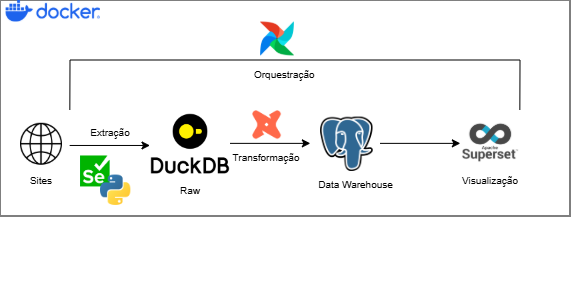
\includegraphics[width=1.0\linewidth]{img/arquitetura.png}
    \caption{Arquitetura completa do pipeline de dados}
    \label{fig:arquitetura}
\end{figure}

Para a fase crucial de aquisição e extração de conteúdo dinâmico (\textit{web scraping}), a ferramenta central adotada foi o \textbf{Selenium WebDriver}. Este framework de automação de navegadores serviu como a espinha dorsal da solução, simulando o comportamento de um usuário real (como cliques, rolagem de página e interações complexas com elementos de interface, utilizando recursos da biblioteca que permitem simular ações do mouse e selecionar opções em menus suspensos). Sua capacidade de lidar com interações complexas garante a extração de dados de fontes que demandam alta flexibilidade de acesso.

Uma vez extraídos, os dados brutos foram imediatamente direcionados para o \textbf{DuckDB}, que atuou como repositório temporário de alto desempenho. O DuckDB é um sistema de banco de dados relacional e analítico que se destaca por sua arquitetura embutida, ou seja, ele funciona diretamente dentro do programa que o utiliza, sem a necessidade de instalar ou manter um servidor de banco de dados separado. Essa característica simplifica a arquitetura do projeto e minimiza os custos indiretos associados à complexidade operacional e manutenção de um componente dedicado.

Após a ingestão inicial, os dados brutos foram migrados para o \textbf{PostgreSQL}, um sistema de gerenciamento de banco de dados relacional open source que atua como o DW analítico do projeto. Diferentemente do DuckDB, o PostgreSQL opera no modelo cliente-servidor, o que siganifica que ele funciona como um serviço independente ao qual múltiplas ferramentas podem se conectar simultaneamente, uma característica essencial para a integração com as demais tecnologias do pipeline. Sua robustez, ampla conformidade com padrões SQL e mais de 35 anos de desenvolvimento ativo o consolidam como uma das soluções open source mais confiáveis para cargas analíticas.

Para a camada de transformação dos dados, foi adotado o \ac{dbt}, uma ferramenta open source que implementa o paradigma de transformação como código (\textit{transformation as code}). Em termos práticos, isso significa que todas as regras de limpeza, padronização e reorganização dos dados são escritas em SQL, a linguagem padrão para consultas em bancos de dados, e armazenadas em arquivos versionáveis, da mesma forma que se versiona o código de um software. O dbt opera exclusivamente sobre os dados já carregados no PostgreSQL, alinhando-se à abordagem ELT discutida no Capítulo 2. Seu sistema integrado de testes automáticos e documentação agrega uma camada de qualidade e governança que seria difícil de replicar com scripts avulsos.

A orquestração de todo o pipeline, desde a execução dos scripts de web scraping até a materialização dos modelos dbt, foi confiada ao \textbf{Apache Airflow}, uma plataforma open source de gerenciamento de fluxos de trabalho. O Airflow permite a definição de pipelines como código Python, utilizando o conceito de \acs{dags}, que são grafos direcionados sem ciclos nos quais cada nó representa uma tarefa a ser executada e as setas entre eles definem a ordem de execução, ou seja, qual tarefa precisa terminar antes que a próxima comece. Sua interface web oferece visibilidade completa sobre o histórico de execuções, registros detalhados de cada etapa e mecanismos automáticos de reexecução em caso de falha, garantindo a observabilidade e a resiliência do pipeline em produção.

Por fim, a disponibilização dos dados transformados para análise visual foi realizada por meio do \textbf{Apache Superset}, uma plataforma open source de \acs{bi} que permite a criação de painéis interativos (\textit{dashboards}) e a exploração de dados via consultas SQL. O Superset conecta-se nativamente ao PostgreSQL e se posiciona como uma alternativa direta a ferramentas proprietárias como Tableau e Power BI, sem custos de licenciamento.

Em paralelo, o processamento e a qualidade dos dados foram aprimorados pelo uso estratégico de bibliotecas nativas do Python. A biblioteca de expressões regulares foi essencial na etapa de transformação para identificar e extrair padrões específicos dentro de textos, como valores monetários e durações de viagem que estavam misturados em frases descritivas. Adicionalmente, bibliotecas auxiliares foram integradas ao pipeline para gerenciar a organização dos arquivos e enriquecer os dados com informações temporais (como a data e hora da coleta), garantindo a rastreabilidade e a consistência do conjunto de dados final.

\section{Tentativa com a ferramenta Browser Use}

Antes de iniciar a abordagem manual com o Selenium, foi explorada a possibilidade de usar ferramentas de inteligência artificial para a extração de dados. A ferramenta Browser Use, que atua como um agente de navegação autônomo, prometia uma alternativa mais intuitiva e menos dependente de seletores CSS fixos, ao permitir a automação de tarefas online em linguagem natural. Essa abordagem era perfeitamente alinhada com a premissa do trabalho, que busca soluções \acs{open_source} e flexíveis. O agente foi configurado para usar o modelo de linguagem Mistral, que rodou localmente via Ollama e foi orquestrado com a biblioteca LangChain.

O Mistral 8x7B é um Grande Modelo de Linguagem (\ac{llm}) notável por sua arquitetura Mixture of Experts (MoE), sendo composto por oito módulos especialistas, cada um contendo sete bilhões de parâmetros. Essa estrutura é projetada para especializar-se em diferentes tipos de tarefas e está na vanguarda da pesquisa em aprendizado multimodal, visando aprimorar a integração e o processamento de dados de texto, imagem e áudio.

A tentativa demonstrou que o \textit{Browser Use} é funcional. O modelo conseguia interagir com as páginas e extrair informações, validando a promessa de que é possível automatizar o processo com comandos de alto nível. No entanto, essa abordagem enfrentou uma limitação técnica significativa: o processamento local do modelo de IA. A execução do Mistral via Ollama se mostrou extremamente intensiva em termos de recursos computacionais, sobrecarregando a máquina utilizada para o projeto.

Os testes foram realizados em um computador DESKTOP-I0H93GR, equipado com um processador \textit{AMD Ryzen 7 4800HS with Radeon Graphics} (2,90 GHz), 16 GB de memória RAM (15,4 GB utilizáveis) e sistema operacional Windows 10 de 64 bits. Apesar de possuir boas especificações para tarefas gerais de desenvolvimento, a execução local do modelo exigiu recursos acima da capacidade disponível, resultando em lentidão significativa e, em alguns casos, no desligamento completo do computador devido à alta demanda de CPU e memória RAM.

Essa limitação inviabilizou a continuidade do projeto com essa arquitetura, evidenciando a necessidade de recursos computacionais mais robustos ou da adoção de uma abordagem baseada em infraestrutura em nuvem para o processamento de modelos de linguagem de grande porte.

Essa experiência reforça a importância de considerar o custo operacional e os requisitos de infraestrutura ao escolher as ferramentas para um \textit{pipeline} de dados, especialmente em projetos que buscam a acessibilidade e a eficiência. A tentativa, embora não tenha sido bem-sucedida em termos de implementação prática devido às limitações de \textit{hardware}, serviu como uma valiosa lição sobre as barreiras que ainda existem para o uso de soluções de IA em ambientes de baixo custo, destacando que essa abordagem é promissora para o futuro, desde que haja um \textit{hardware} mais potente à disposição.

\label{sec:conclusao}

\chapter{Conclusão}


Apesar do avanço das tecnologias \ac{open_source} nas últimas décadas, muitas instituições ainda apresentam uma certa resistência em incorporar essas soluções em lugar das ferramentas proprietárias. Fatores relacionados à assistência técnica, à confiabilidade, à segurança, à continuidade, manutenção e à complexidade de implementação muitas vezes levam a gestores a escolher plataformas comerciais, mesmo diante dos altos custos de licenciamento.

A análise da literatura efetuada neste estudo evidenciou que o ecossistema \ac{open_source} conta, atualmente, com uma grande quantidade de ferramentas para todas as fases de um pipeline de dados. Tecnologias como Apache Kafka, Apache Airflow, Apache Spark, Apache NiFi, HDFS e Apache Superset são amplamente empregadas, proporcionando funcionalidades equivalentes às disponíveis em várias soluções proprietárias. Entretanto, as pesquisas também demonstram que a implementação dessas tecnologias não se configura como uma tarefa simples, demandando conhecimento técnico, integração entre diversos componentes, definição de arquiteturas e um esforço adicional para configuração e manutenção. Assim, a grande quantidade de ferramentas acessíveis pode constituir um obstáculo para organizações que almejam implementar iniciativas de ED com base unicamente em tecnologias \ac{open_source}.

Visando auxiliar na diminuição dessa barreira, esta pesquisa apresentou uma proposta de arquitetura de pipeline de dados fundamentada em ferramentas \ac{open_source}, elaborada com base nos resultados da revisão da literatura e concretizada através de um protótipo funcional. A arquitetura sugerida evidenciou a possibilidade de combinar diversas tecnologias \ac{open_source} para criar uma solução integrada e eficiente, capaz de atender às necessidades de um processo de dados completo.


\section{Ameaças à Validade}

Fazendo uma análise crítica dos resultados e conclusões deste trabalho, é importante reconhecer as principais ameaças à validade que podem impactar a interpretação dos achados apresentados. Essas ameaças estão relacionadas a diferentes aspectos do processo de pesquisa e desenvolvimento, incluindo a forma como os dados foram coletados, analisados e interpretados, bem como a generalização dos resultados para outros contextos \cite[]{ihantola2011threats}.

\begin{itemize}

\item \textbf{Validade de Conclusão:}  As conclusões deste trabalho foram fundamentadas principalmente na revisão da literatura e na implementação de um protótipo funcional. Não sendo realizados experimentos controlados, \textit{benchmarks} de desempenho ou estudos comparativos que permitissem mensurar quantitativamente aspectos como escalabilidade, confiabilidade, custo operacional ou desempenho da arquitetura proposta. Dessa forma, as conclusões devem ser interpretadas como evidências de viabilidade técnica e não como comprovação definitiva.


\item \textbf{Validade Interna :} O protótipo foi desenvolvido em um ambiente controlado e utilizando um conjunto específico de fontes de dados relacionadas ao setor de turismo. A ausência de comparação direta com arquiteturas proprietárias ou outras arquiteturas open source limita a capacidade de atribuir os resultados exclusivamente às tecnologias selecionadas. Além disso, fatores como configuração de hardware, infraestrutura disponível e características particulares das fontes de dados podem influenciar os resultados obtidos durante a implementação.

\item \textbf{Validade de Construção:} A arquitetura proposta foi construída com base nos resultados da revisão rápida da literatura e em um cenário motivador de coleta de dados turísticos. Entretanto, o protótipo não contempla todos os desafios encontrados em ambientes produtivos, tais como processamento de grandes volumes de dados, alta disponibilidade, recuperação de desastres, monitoramento avançado, segurança corporativa e governança de dados. Dessa forma, existe o risco de que algumas simplificações adotadas durante o desenvolvimento não representem integralmente a complexidade encontrada em ambientes reais de produção.

\item \textbf{Validade Externa:}   O cenário utilizado concentrou-se na coleta de dados de websites de turismo internacional, podendo apresentar características distintas de outros domínios de aplicação da ED.
Embora as ferramentas selecionadas sejam amplamente utilizadas no ecossistema de \textit{Big Data}, diferentes organizações podem possuir requisitos específicos relacionados a volume de dados, infraestrutura, governança, requisitos regulatórios e restrições operacionais.
\end{itemize}

Por fim, destaca-se que a realização de uma avaliação experimental formal não fez parte do escopo deste Trabalho de Conclusão de Curso. O objetivo principal foi identificar, por meio da literatura, ferramentas open source relevantes para pipelines de dados, propor uma arquitetura baseada nesses achados e demonstrar sua viabilidade por meio da implementação de um protótipo funcional. Como trabalhos futuros, recomenda-se a realização de benchmarks de desempenho, comparações com soluções proprietárias e estudos de caso em ambientes reais de produção.


\label{bibpage}
\addcontentsline{toc}{section}{Referências Bibliográficas}
\bibliography{references}
\bibliographystyle{plainnat}
\label{bibfinalpage}

\label{lastpage}
\end{document}